
%% bare_jrnl.tex
%% V1.3
%% 2007/01/11
%% by Michael Shell
%% see http://www.michaelshell.org/
%% for current contact information.
%%
%% This is a skeleton file demonstrating the use of IEEEtran.cls
%% (requires IEEEtran.cls version 1.7 or later) with an IEEE journal paper.
%%
%% Support sites:
%% http://www.michaelshell.org/tex/ieeetran/
%% http://www.ctan.org/tex-archive/macros/latex/contrib/IEEEtran/
%% and
%% http://www.ieee.org/



% *** Authors should verify (and, if needed, correct) their LaTeX system  ***
% *** with the testflow diagnostic prior to trusting their LaTeX platform ***
% *** with production work. IEEE's font choices can trigger bugs that do  ***
% *** not appear when using other class files.                            ***
% The testflow support page is at:
% http://www.michaelshell.org/tex/testflow/


%%*************************************************************************
%% Legal Notice:
%% This code is offered as-is without any warranty either expressed or
%% implied; without even the implied warranty of MERCHANTABILITY or
%% FITNESS FOR A PARTICULAR PURPOSE! 
%% User assumes all risk.
%% In no event shall IEEE or any contributor to this code be liable for
%% any damages or losses, including, but not limited to, incidental,
%% consequential, or any other damages, resulting from the use or misuse
%% of any information contained here.
%%
%% All comments are the opinions of their respective authors and are not
%% necessarily endorsed by the IEEE.
%%
%% This work is distributed under the LaTeX Project Public License (LPPL)
%% ( http://www.latex-project.org/ ) version 1.3, and may be freely used,
%% distributed and modified. A copy of the LPPL, version 1.3, is included
%% in the base LaTeX documentation of all distributions of LaTeX released
%% 2003/12/01 or later.
%% Retain all contribution notices and credits.
%% ** Modified files should be clearly indicated as such, including  **
%% ** renaming them and changing author support contact information. **
%%
%% File list of work: IEEEtran.cls, IEEEtran_HOWTO.pdf, bare_adv.tex,
%%                    bare_conf.tex, bare_jrnl.tex, bare_jrnl_compsoc.tex
%%*************************************************************************

% Note that the a4paper option is mainly intended so that authors in
% countries using A4 can easily print to A4 and see how their papers will
% look in print - the typesetting of the document will not typically be
% affected with changes in paper size (but the bottom and side margins will).
% Use the testflow package mentioned above to verify correct handling of
% both paper sizes by the user's LaTeX system.
%
% Also note that the "draftcls" or "draftclsnofoot", not "draft", option
% should be used if it is desired that the figures are to be displayed in
% draft mode.
%
\documentclass[journal]{journal}

\newtheorem{algorithm}{Algorithm}
\usepackage{algpseudocode}
\usepackage{varwidth}
\usepackage{graphicx}
\usepackage{amsmath}
\usepackage{color}
\usepackage{url}
\graphicspath{{./images}}

%
% If IEEEtran.cls has not been installed into the LaTeX system files,
% manually specify the path to it like:
% \documentclass[journal]{../sty/IEEEtran}


\ifCLASSINFOpdf
  % \usepackage[pdftex]{graphicx}
  % declare the path(s) where your graphic files are
  % \graphicspath{{../pdf/}{../jpeg/}}
  % and their extensions so you won't have to specify these with
  % every instance of \includegraphics
  % \DeclareGraphicsExtensions{.pdf,.jpeg,.png}
\else
  % or other class option (dvipsone, dvipdf, if not using dvips). graphicx
  % will default to the driver specified in the system graphics.cfg if no
  % driver is specified.
  % \usepackage[dvips]{graphicx}
  % declare the path(s) where your graphic files are
  % \graphicspath{{../eps/}}
  % and their extensions so you won't have to specify these with
  % every instance of \includegraphics
  % \DeclareGraphicsExtensions{.eps}
\fi



% Some very useful LaTeX packages include:
% (uncomment the ones you want to load)


% *** MISC UTILITY PACKAGES ***
%
%\usepackage{ifpdf}
% Heiko Oberdiek's ifpdf.sty is very useful if you need conditional
% compilation based on whether the output is pdf or dvi.
% usage:
% \ifpdf
%   % pdf code
% \else
%   % dvi code
% \fi
% The latest version of ifpdf.sty can be obtained from:
% http://www.ctan.org/tex-archive/macros/latex/contrib/oberdiek/
% Also, note that IEEEtran.cls V1.7 and later provides a builtin
% \ifCLASSINFOpdf conditional that works the same way.
% When switching from latex to pdflatex and vice-versa, the compiler may
% have to be run twice to clear warning/error messages.






% *** CITATION PACKAGES ***
%
%\usepackage{cite}
% cite.sty was written by Donald Arseneau
% V1.6 and later of IEEEtran pre-defines the format of the cite.sty package
% \cite{} output to follow that of IEEE. Loading the cite package will
% result in citation numbers being automatically sorted and properly
% "compressed/ranged". e.g., [1], [9], [2], [7], [5], [6] without using
% cite.sty will become [1], [2], [5]--[7], [9] using cite.sty. cite.sty's
% \cite will automatically add leading space, if needed. Use cite.sty's
% noadjust option (cite.sty V3.8 and later) if you want to turn this off.
% cite.sty is already installed on most LaTeX systems. Be sure and use
% version 4.0 (2003-05-27) and later if using hyperref.sty. cite.sty does
% not currently provide for hyperlinked citations.
% The latest version can be obtained at:
% http://www.ctan.org/tex-archive/macros/latex/contrib/cite/
% The documentation is contained in the cite.sty file itself.






% *** GRAPHICS RELATED PACKAGES ***
%
%\ifCLASSINFOpdf
  % \usepackage[pdftex]{graphicx}
  % declare the path(s) where your graphic files are
  % \graphicspath{{../pdf/}{../jpeg/}}
  % and their extensions so you won't have to specify these with
  % every instance of \includegraphics
  % \DeclareGraphicsExtensions{.pdf,.jpeg,.png}
%\else
  % or other class option (dvipsone, dvipdf, if not using dvips). graphicx
  % will default to the driver specified in the system graphics.cfg if no
  % driver is specified.
  % \usepackage[dvips]{graphicx}
  % declare the path(s) where your graphic files are
  % \graphicspath{{../eps/}}
  % and their extensions so you won't have to specify these with
  % every instance of \includegraphics
  % \DeclareGraphicsExtensions{.eps}
%\fi
% graphicx was written by David Carlisle and Sebastian Rahtz. It is
% required if you want graphics, photos, etc. graphicx.sty is already
% installed on most LaTeX systems. The latest version and documentation can
% be obtained at: 
% http://www.ctan.org/tex-archive/macros/latex/required/graphics/
% Another good source of documentation is "Using Imported Graphics in
% LaTeX2e" by Keith Reckdahl which can be found as epslatex.ps or
% epslatex.pdf at: http://www.ctan.org/tex-archive/info/
%
% latex, and pdflatex in dvi mode, support graphics in encapsulated
% postscript (.eps) format. pdflatex in pdf mode supports graphics
% in .pdf, .jpeg, .png and .mps (metapost) formats. Users should ensure
% that all non-photo figures use a vector format (.eps, .pdf, .mps) and
% not a bitmapped formats (.jpeg, .png). IEEE frowns on bitmapped formats
% which can result in "jaggedy"/blurry rendering of lines and letters as
% well as large increases in file sizes.
%
% You can find documentation about the pdfTeX application at:
% http://www.tug.org/applications/pdftex





% *** MATH PACKAGES ***
%
%\usepackage[cmex10]{amsmath}
% A popular package from the American Mathematical Society that provides
% many useful and powerful commands for dealing with mathematics. If using
% it, be sure to load this package with the cmex10 option to ensure that
% only type 1 fonts will utilized at all point sizes. Without this option,
% it is possible that some math symbols, particularly those within
% footnotes, will be rendered in bitmap form which will result in a
% document that can not be IEEE Xplore compliant!
%
% Also, note that the amsmath package sets \interdisplaylinepenalty to 10000
% thus preventing page breaks from occurring within multiline equations. Use:
%\interdisplaylinepenalty=2500
% after loading amsmath to restore such page breaks as IEEEtran.cls normally
% does. amsmath.sty is already installed on most LaTeX systems. The latest
% version and documentation can be obtained at:
% http://www.ctan.org/tex-archive/macros/latex/required/amslatex/math/





% *** SPECIALIZED LIST PACKAGES ***
%
%\usepackage{algorithmic}
% algorithmic.sty was written by Peter Williams and Rogerio Brito.
% This package provides an algorithmic environment fo describing algorithms.
% You can use the algorithmic environment in-text or within a figure
% environment to provide for a floating algorithm. Do NOT use the algorithm
% floating environment provided by algorithm.sty (by the same authors) or
% algorithm2e.sty (by Christophe Fiorio) as IEEE does not use dedicated
% algorithm float types and packages that provide these will not provide
% correct IEEE style captions. The latest version and documentation of
% algorithmic.sty can be obtained at:
% http://www.ctan.org/tex-archive/macros/latex/contrib/algorithms/
% There is also a support site at:
% http://algorithms.berlios.de/index.html
% Also of interest may be the (relatively newer and more customizable)
% algorithmicx.sty package by Szasz Janos:
% http://www.ctan.org/tex-archive/macros/latex/contrib/algorithmicx/




% *** ALIGNMENT PACKAGES ***
%
%\usepackage{array}
% Frank Mittelbach's and David Carlisle's array.sty patches and improves
% the standard LaTeX2e array and tabular environments to provide better
% appearance and additional user controls. As the default LaTeX2e table
% generation code is lacking to the point of almost being broken with
% respect to the quality of the end results, all users are strongly
% advised to use an enhanced (at the very least that provided by array.sty)
% set of table tools. array.sty is already installed on most systems. The
% latest version and documentation can be obtained at:
% http://www.ctan.org/tex-archive/macros/latex/required/tools/


%\usepackage{mdwmath}
%\usepackage{mdwtab}
% Also highly recommended is Mark Wooding's extremely powerful MDW tools,
% especially mdwmath.sty and mdwtab.sty which are used to format equations
% and tables, respectively. The MDWtools set is already installed on most
% LaTeX systems. The lastest version and documentation is available at:
% http://www.ctan.org/tex-archive/macros/latex/contrib/mdwtools/


% IEEEtran contains the IEEEeqnarray family of commands that can be used to
% generate multiline equations as well as matrices, tables, etc., of high
% quality.


%\usepackage{eqparbox}
% Also of notable interest is Scott Pakin's eqparbox package for creating
% (automatically sized) equal width boxes - aka "natural width parboxes".
% Available at:
% http://www.ctan.org/tex-archive/macros/latex/contrib/eqparbox/





% *** SUBFIGURE PACKAGES ***
%\usepackage[tight,footnotesize]{subfigure}
% subfigure.sty was written by Steven Douglas Cochran. This package makes it
% easy to put subfigures in your figures. e.g., "Figure 1a and 1b". For IEEE
% work, it is a good idea to load it with the tight package option to reduce
% the amount of white space around the subfigures. subfigure.sty is already
% installed on most LaTeX systems. The latest version and documentation can
% be obtained at:
% http://www.ctan.org/tex-archive/obsolete/macros/latex/contrib/subfigure/
% subfigure.sty has been superceeded by subfig.sty.



%\usepackage[caption=false]{caption}
%\usepackage[font=footnotesize]{subfig}
% subfig.sty, also written by Steven Douglas Cochran, is the modern
% replacement for subfigure.sty. However, subfig.sty requires and
% automatically loads Axel Sommerfeldt's caption.sty which will override
% IEEEtran.cls handling of captions and this will result in nonIEEE style
% figure/table captions. To prevent this problem, be sure and preload
% caption.sty with its "caption=false" package option. This is will preserve
% IEEEtran.cls handing of captions. Version 1.3 (2005/06/28) and later 
% (recommended due to many improvements over 1.2) of subfig.sty supports
% the caption=false option directly:
%\usepackage[caption=false,font=footnotesize]{subfig}
%
% The latest version and documentation can be obtained at:
% http://www.ctan.org/tex-archive/macros/latex/contrib/subfig/
% The latest version and documentation of caption.sty can be obtained at:
% http://www.ctan.org/tex-archive/macros/latex/contrib/caption/




% *** FLOAT PACKAGES ***
%
%\usepackage{fixltx2e}
% fixltx2e, the successor to the earlier fix2col.sty, was written by
% Frank Mittelbach and David Carlisle. This package corrects a few problems
% in the LaTeX2e kernel, the most notable of which is that in current
% LaTeX2e releases, the ordering of single and double column floats is not
% guaranteed to be preserved. Thus, an unpatched LaTeX2e can allow a
% single column figure to be placed prior to an earlier double column
% figure. The latest version and documentation can be found at:
% http://www.ctan.org/tex-archive/macros/latex/base/



%\usepackage{stfloats}
% stfloats.sty was written by Sigitas Tolusis. This package gives LaTeX2e
% the ability to do double column floats at the bottom of the page as well
% as the top. (e.g., "\begin{figure*}[!b]" is not normally possible in
% LaTeX2e). It also provides a command:
%\fnbelowfloat
% to enable the placement of footnotes below bottom floats (the standard
% LaTeX2e kernel puts them above bottom floats). This is an invasive package
% which rewrites many portions of the LaTeX2e float routines. It may not work
% with other packages that modify the LaTeX2e float routines. The latest
% version and documentation can be obtained at:
% http://www.ctan.org/tex-archive/macros/latex/contrib/sttools/
% Documentation is contained in the stfloats.sty comments as well as in the
% presfull.pdf file. Do not use the stfloats baselinefloat ability as IEEE
% does not allow \baselineskip to stretch. Authors submitting work to the
% IEEE should note that IEEE rarely uses double column equations and
% that authors should try to avoid such use. Do not be tempted to use the
% cuted.sty or midfloat.sty packages (also by Sigitas Tolusis) as IEEE does
% not format its papers in such ways.


%\ifCLASSOPTIONcaptionsoff
%  \usepackage[nomarkers]{endfloat}
% \let\MYoriglatexcaption\caption
% \renewcommand{\caption}[2][\relax]{\MYoriglatexcaption[#2]{#2}}
%\fi
% endfloat.sty was written by James Darrell McCauley and Jeff Goldberg.
% This package may be useful when used in conjunction with IEEEtran.cls'
% captionsoff option. Some IEEE journals/societies require that submissions
% have lists of figures/tables at the end of the paper and that
% figures/tables without any captions are placed on a page by themselves at
% the end of the document. If needed, the draftcls IEEEtran class option or
% \CLASSINPUTbaselinestretch interface can be used to increase the line
% spacing as well. Be sure and use the nomarkers option of endfloat to
% prevent endfloat from "marking" where the figures would have been placed
% in the text. The two hack lines of code above are a slight modification of
% that suggested by in the endfloat docs (section 8.3.1) to ensure that
% the full captions always appear in the list of figures/tables - even if
% the user used the short optional argument of \caption[]{}.
% IEEE papers do not typically make use of \caption[]'s optional argument,
% so this should not be an issue. A similar trick can be used to disable
% captions of packages such as subfig.sty that lack options to turn off
% the subcaptions:
% For subfig.sty:
% \let\MYorigsubfloat\subfloat
% \renewcommand{\subfloat}[2][\relax]{\MYorigsubfloat[]{#2}}
% For subfigure.sty:
% \let\MYorigsubfigure\subfigure
% \renewcommand{\subfigure}[2][\relax]{\MYorigsubfigure[]{#2}}
% However, the above trick will not work if both optional arguments of
% the \subfloat/subfig command are used. Furthermore, there needs to be a
% description of each subfigure *somewhere* and endfloat does not add
% subfigure captions to its list of figures. Thus, the best approach is to
% avoid the use of subfigure captions (many IEEE journals avoid them anyway)
% and instead reference/explain all the subfigures within the main caption.
% The latest version of endfloat.sty and its documentation can obtained at:
% http://www.ctan.org/tex-archive/macros/latex/contrib/endfloat/
%
% The IEEEtran \ifCLASSOPTIONcaptionsoff conditional can also be used
% later in the document, say, to conditionally put the References on a 
% page by themselves.





% *** PDF, URL AND HYPERLINK PACKAGES ***
%
%\usepackage{url}
% url.sty was written by Donald Arseneau. It provides better support for
% handling and breaking URLs. url.sty is already installed on most LaTeX
% systems. The latest version can be obtained at:
% http://www.ctan.org/tex-archive/macros/latex/contrib/misc/
% Read the url.sty source comments for usage information. Basically,
% \url{my_url_here}.





% *** Do not adjust lengths that control margins, column widths, etc. ***
% *** Do not use packages that alter fonts (such as pslatex).         ***
% There should be no need to do such things with IEEEtran.cls V1.6 and later.
% (Unless specifically asked to do so by the journal or conference you plan
% to submit to, of course. )


% correct bad hyphenation here
%
% paper title
% can use linebreaks \\ within to get better formatting as desired

%
%
% author names and IEEE memberships
% note positions of commas and nonbreaking spaces ( ~ ) LaTeX will not break
% a structure at a ~ so this keeps an author's name from being broken across
% two lines.
% use \thanks{} to gain access to the first footnote area
% a separate \thanks must be used for each paragraph as LaTeX2e's \thanks
% was not built to handle multiple paragraphs
%

% This is "sig-alternate.tex" V2.0 May 2012
% This file should be compiled with V2.5 of "sig-alternate.cls" May 2012
%
% This example file demonstrates the use of the 'sig-alternate.cls'
% V2.5 LaTeX2e document class file. It is for those submitting
% articles to ACM Conference Proceedings WHO DO NOT WISH TO
% STRICTLY ADHERE TO THE SIGS (PUBS-BOARD-ENDORSED) STYLE.
% The 'sig-alternate.cls' file will produce a similar-looking,
% albeit, 'tighter' paper resulting in, invariably, fewer pages.
%
% ----------------------------------------------------------------------------------------------------------------
% This .tex file (and associated .cls V2.5) produces:
%       1) The Permission Statement
%       2) The Conference (location) Info information
%       3) The Copyright Line with ACM data
%       4) NO page numbers
%
% as against the acm_proc_article-sp.cls file which
% DOES NOT produce 1) thru' 3) above.
%
% Using 'sig-alternate.cls' you have control, however, from within
% the source .tex file, over both the CopyrightYear
% (defaulted to 200X) and the ACM Copyright Data
% (defaulted to X-XXXXX-XX-X/XX/XX).
% e.g.
% \CopyrightYear{2007} will cause 2007 to appear in the copyright line.
% \crdata{0-12345-67-8/90/12} will cause 0-12345-67-8/90/12 to appear in the copyright line.
%
% ---------------------------------------------------------------------------------------------------------------
% This .tex source is an example which *does* use
% the .bib file (from which the .bbl file % is produced).
% REMEMBER HOWEVER: After having produced the .bbl file,
% and prior to final submission, you *NEED* to 'insert'
% your .bbl file into your source .tex file so as to provide
% ONE 'self-contained' source file.
%
% ================= IF YOU HAVE QUESTIONS =======================
% Questions regarding the SIGS styles, SIGS policies and
% procedures, Conferences etc. should be sent to
% Adrienne Griscti (griscti@acm.org)
%
% Technical questions _only_ to
% Gerald Murray (murray@hq.acm.org)
% ===============================================================
%
% For tracking purposes - this is V2.0 - May 2012



\begin{document}


% ISBN

%Conference

%
% --- Author Metadata here ---
%\conferenceinfo{WOODSTOCK}{'97 El Paso, Texas USA}
%
% --- Author Metadata here ---
%\conferenceinfo{WOODSTOCK}{'97 El Paso, Texas USA}
%\CopyrightYear{2007} % Allows default copyright year (20XX) to be over-ridden - IF NEED BE.
%\crdata{0-12345-67-8/90/01}  % Allows default copyright data (0-89791-88-6/97/05) to be over-ridden - IF NEED BE.
% --- End of Author Metadata ---

\title{Scalable Learning of Tree-Based Models on Sparsely Representable Data}
%
% You need the command \numberofauthors to handle the 'placement
% and alignment' of the authors beneath the title.
%
% For aesthetic reasons, we recommend 'three authors at a time'
% i.e. three 'name/affiliation blocks' be placed beneath the title.
%
% NOTE: You are NOT restricted in how many 'rows' of
% "name/affiliations" may appear. We just ask that you restrict
% the number of 'columns' to three.
%
% Because of the available 'opening page real-estate'
% we ask you to refrain from putting more than six authors
% (two rows with three columns) beneath the article title.
% More than six makes the first-page appear very cluttered indeed.
%
% Use the \alignauthor commands to handle the names
% and affiliations for an 'aesthetic maximum' of six authors.
% Add names, affiliations, addresses for
% the seventh etc. author(s) as the argument for the
% \additionalauthors command.
% These 'additional authors' will be output/set for you
% without further effort on your part as the last section in
% the body of your article BEFORE References or any Appendices.

 %  in this sample file, there are a *total*
% of EIGHT authors. SIX appear on the 'first-page' (for formatting
% reasons) and the remaining two appear in the \additionalauthors section.
%

% You can go ahead and credit any number of authors here,
% e.g. one 'row of three' or two rows (consisting of one row of three
% and a second row of one, two or three).
%
% The command \alignauthor (no curly braces needed) should
% precede each author name, affiliation/snail-mail address and
% e-mail address. Additionally, tag each line of
% affiliation/address with \affaddr, and tag the
% e-mail address with \email.
%
% 1st. author

\author{
Fares Hedayati,~{upwork},~{fares19@upwork.com}

Arnauld Joly, ~{University of Li{e}ge},~{a.joly@ulg.ac.be}
Panagiotis Papadimitriou,~{upwork},~{papadimitriou@upwork.com}}
% There's nothing stopping you putting the seventh, eighth, etc.
% author on the opening page (as the 'third row') but we ask,
% for aesthetic reasons that you place these 'additional authors'
% in the \additional authors block, viz.
\date{19 May 2016}


\maketitle
\thispagestyle{empty}

\begin{abstract}
Many machine learning tasks such as text annotation usually require
  training over very big datasets, e.g., millions of web documents,
  that can be represented in a sparse input space. State-of-the-art
  tree-based ensemble algorithms cannot scale to such datasets, since
  they include operations whose running time is a function of the
  input space size rather than a function of the non-zero input
  elements. 
  In this paper, we propose an efficient splitting algorithm to
  leverage input sparsity within decision tree
  methods. 
  Our algorithm improves training time over sparse datasets by more
  than two orders of magnitude and it has been incorporated in the current
  version of \emph{scikit-learn}\footnote{http://scikit-learn.org},
  the most popular open source Python machine learning library.
  \end{abstract}

% A category with the (minimum) three required fields
%\category{Decision Trees}
%A category including the fourth, optional field follows...
%\category{Big Data, Scalable methods}

%\terms{Algorithms, Experimentation, Performance}

\keywords{machine learning, classification trees, regression trees, sparse data, scalability}

\input{intro.tex}
\section{Decision Trees With Dense Input Data} \label{sec:background}
\subsection{Notation}

We denote by $\mathcal{X}$ an input space and by $\mathcal{Y}$ the output space.
Without loss of generality, we suppose that $\mathcal{X} = \mathcal{R}^m$ where
$m$ denotes the number of features and $\mathcal{Y} = \mathcal{R}$ in case of regression or $\mathcal{Y} = \{0, 1, \cdots, K-1\}$ in case of a $K$-$class$ classification. Learning samples are represented by a pair of matrices
$(X, Y) \subseteq (\mathcal{X}, \mathcal{Y})_{i=0}^{n-1}$ with $n$ rows, where each row
corresponds to a sample and each column to a feature or an output variable. 
In the process of decision tree induction we have to move samples around, instead of moving the actual rows of $(X,Y)$ we move their indices. For this purpose we introduce $\mathcal{L} = [0, 1, \cdots , n-1]$ which is the list of row indices of $(X,Y)$. As we will see in the next section, impurity measure plays a crucial role in induction of decision trees. An impurity measure of a set of samples $\mathcal{L}$ measures the heterogeneity of the target variable of the samples. The variance of the target variable is used in regression, and Gini and cross-entropy are usually used in tree-based classification algorithms. Given $\mathcal{L}$, we let $\hat{p}_k$ be the empirical probability of class $k$ in the dataset. The Gini impurity measure is defined as: 
\begin{equation}
\label{gini}
I(\mathcal{L}) = \sum_{k=0}^{K-1} \hat{p}_k \left(1- \hat{p}_k\right), 
\end{equation}
and the cross-entropy impurity measure is defined as: 
\begin{equation}
\label{entropy}
I(\mathcal{L}) = \sum_{k=0}^{K-1} \hat{p}_k \log\left(\hat{p}_k\right)
\end{equation}
Note that the impurity measure is maximized in case of uniform distribution of the target variable which makes $\mathcal{L}$ most heterogenous, i.e. $\hat{p}_k = \frac{1}{K}$. Moreover the impurity measure is minimized when the empirical probability is concentrated on one class while other classes have $\hat{p}_k = 0$. 

\subsection{Training}

	A decision tree \cite{breiman1984classification} is built by recursively
splitting the sample set into two nodes by maximizing the average reduction of an impurity measure: 
\begin{equation}
\label{red}
\Delta{}I(s, \mathcal{L}) =
\left(I({ \mathcal{L}}) - \left(
\frac{|\mathcal{L}_r|}{|\mathcal{L}|} I({\mathcal{L}_r}) +
\frac{|\mathcal{L}_l|}{|\mathcal{L}|} I({\mathcal{L}_l})\right)\right)
\end{equation}
where $s=\left(j, \, \theta\right)$ is a splitting rule composed of a feature index $j$ and a threshold value $\theta$ which divides the sample set into $ \mathcal{L}_l$ and $ \mathcal{L}_r$ where 
\begin{equation}
\label{left}
\mathcal{L}_l = \{ i \in \mathcal{L} \, | \, X_{i,j} < \theta  \}, 
\end{equation}
and 
\begin{equation}
\label{right}
\mathcal{L}_r = \{ i \in \mathcal{L} \, | \, X_{i,j} \ge \theta  \}
\end{equation}
This recursive procedure is repeated until a stopping condition is met, e.g. a maximal depth
is reached or there are too few samples to split. Those stopping criteria act
as regularization parameters. Leaves are labeled by the output mean in
regression or by the class frequencies in classification with reaching training
samples. The recursive induction of the decision decision is described
by Algorithm~\ref{tree_induction} and the search for the best split
is described by Algorithm~\ref{find_best_split}. Note that sorting samples (Line~\ref{line_sorting}) in a node along different features is at the core of Algorithm~\ref{find_best_split}; it speeds up computation of the impurity measure for all possible splitting rules in an incremental manner. In Algorithm~\ref{tree_induction} below a stack is initially setup with a single element namely a pair of a root $t_0$ and the entire set of samples $\mathcal{L}$ (Line~5). Line~7 pops the next set of samples from the stack ($\mathcal{L}_p$) and split it into two nodes, the left node $\mathcal{L}_l$ and and the right node $\mathcal{L}_r$, based on the best splitting rule obtained in Line~11. Note that this splitting is carried out recursively until the stopping criterion are met (Line~8,9) in which case the current node becomes a leaf.

In the context of ensemble, trees are further randomized by searching for the
best split among $k$ features at each node and also might be induced on a
bootstrap copy of the samples. The tree can be grown alternatively in a best-first
search manner by replacing the stack of Algorithm~\ref{tree_induction}
by a priority queue where priority is defined by expected impurity reduction. 

\begin{algorithm}\label{tree_induction}
Build a decision tree
\textnormal{
\begin{algorithmic}[1]
\Function{InduceDecisionTree}{$\mathcal{L}$, $X$, $Y$}
    \State Initialize a tree structure $\tau$ with root node $t_0$
    \State Initialize an empty stack $stack$
    \State Initialize a sample set $\mathcal{L}=\{0,\ldots,n-1\}$
    \State $stack$\Call{.push}{($t_0$, $\mathcal{L}$)}
    \While{$stack$ is not empty}
        \State $t_p$, $\mathcal{L}_p$ = $stack$\Call{.pop}{}()
        \If{$t_p$ satisfies stopping criterion}
            \State Make $t_p$ a leaf node using $\mathcal{L}_p$ and $Y$.
        \Else
            \State \begin{varwidth}[t]{0.8\linewidth}
                   Find a splitting rule $s^*$ which maximizes impurity reduction
                   among possible splitting rules: \\\\%$Q(\mathcal{L}_p, X)$:\\\\
                   $
                   s^* =  {FindBestSplit}(\mathcal{L}_p)\\
                   %\arg\max_{s \in Q(\mathcal{L}_p, X)} \Delta{}I(s, \mathcal{L}_p).
                   $
                   \end{varwidth}
            %\State Make $t_p$ an internal node by splitting rule $s^*$.
            \State Partition $\mathcal{L}_p$ into $\mathcal{L}_r$ and
                   $\mathcal{L}_l$ given $s^*$. \label{line_partition}
            \State Create two empty nodes $t_l$ and $t_r$
            \State Set $t_l$ and $t_r$ the left and right children of $t_p$.
            \State $stack$\Call{.push}{($t_r$, $\mathcal{L}_r$)}
            \State $stack$\Call{.push}{($t_l$, $\mathcal{L}_l$)}
        \EndIf
    \EndWhile
    \State \Return $\tau$
\EndFunction
\end{algorithmic}
}
\end{algorithm}


\subsection{The Optimal Split}

	Given a set of samples $\mathcal{L}_p$ the best splitting rule is computed by finding for each feature a threshold that can reduce the average impurity measure (Equation~\ref{red}) the most and at the end picking the feature with its corresponding optimal threshold that has the best reduction among all features. For a given splitting rule $s = \left(j , \theta\right)$, the whole sample set needs to be traversed once for determining where each sample row belongs to, to the left (Equation~\ref{left}) or to the right node (Equation~\ref{right}). To avoid multiple traversals, for a given feature $j$, the samples are sorted along the feature in an ascending order, and the impurity reduction is computed in an incremental way from the lowest value of feature $j$ to the highest value, treating each feature value as a threshold. As an example consider computing the impurity measure Gini (Equation~\ref{gini}) for all values of feature $j$. We can easily update Equation \ref{red} by keeping track of left node  $\mathcal{L}_l$ and right node  $\mathcal{L}_r$ class frequencies and updating them as we move from one threshold to the next, e.g. from $\theta = X_{i,j}$ to $\theta = X_{i+1,j}$. In other words $\Delta{}I\left(s = (j,X_{i+1,j}), \mathcal{L}\right)$ can be easily computed by updating left node and right node class frequencies for $\theta = X_{i,j}$, and on top of them the empirical probabilities $\hat{p}_k$ and $|\mathcal{L}_l|$ and $|\mathcal{L}_r|$ of Equation~\ref{red}. \\
	
	In Algorithm~\ref{find_best_split} below, Line~3 iterates over all features ranging from $0$ to $m$ creating a dataset $\mathcal{F}_j$ for each one of them. $\mathcal{F}_j$ is basically a collection of all values in column $j$ of the current node $\mathcal{L}_p$. The algorithm computes the impurity for each of the possible values in $\mathcal{F}_j$ in Lines~6 to 8. Line~10 keeps track of the best impurity reduction, and the corresponding rule (referred to $s^*$ in Line~11) which is a combination of a feature index $j$ and a threshold $\theta$. $s^*$ is the returned value of the algorithm and the best splitting rule.   %For more details of this algorithm refer to Algorithm~\ref{find_best_split} below. 



\begin{algorithm}\label{find_best_split}
Search for the best split
\textnormal{
\begin{algorithmic}[1]
\Function{FindBestSplit}{X, $\mathcal{L}_p$}
    \State $\text{best} = -\infty$
    \For{$j \in \{0, \ldots, m-1\}$}
        \State Extract feature values reaching the node
               \[
               \mathcal{F}_j = \{X_{i,j}, \forall i \in \mathcal{L}_p\}.
               \] \label{alg-line:value-extract}
        \State Sort $\mathcal{L}_p$ and $\mathcal{F}_j$ by increasing values
               of $\mathcal{F}_j$.  \label{line_sorting}
	%\State Generate all possible splitting rules
            %   \[
               %Q(\mathcal{F}_j)=\{((x_j \leq \nu), (x_j > \nu))| \nu�\in�\mathcal{F}_j)
               %\]
        %\For{$s$ in $Q(\mathcal{F}_j)$}
        \For{$\theta$ in ${F}_j$}
            \State $s$ = $\left(j, \theta\right)$
            \State Evaluate impurity reduction $s$
                   \[
                   \text{score} = \Delta{}I(s, \mathcal{L}_p).
                   \]
            \If{$\text{score} > \text{best}$}
                \State $\text{best} =\text{score}$
                \State $s^* = s$
            \EndIf
        \EndFor
    \EndFor
    \State \Return $s^*$
\EndFunction
\end{algorithmic}
}
\end{algorithm}

\section{Decision Trees With Sparse Input Data} \label{sec:sparse-input-dt}

\subsection{Sparse matrix format}

For memory efficiency and taking advantage of sparsity we use a data structure
called compressed sparse column (csc) matrix. It is a general format to
represent compactly sparse matrices using three arrays: a $data$ array that stores
the value of each nonzero element for each column, an $indices$ array that stores the row indices
of nonzero elements for each column and an $indptr$ array which stores the beginning and
end of each column in the $data$ and the $indices$ arrays. The row indices of non-zero data points of column $c$ are stored in $indices[indptr[c]$:$indptr[c+1]]$ with their corresponding non-zero values stored in $data[indptr[c]$:$indptr[c+1]]$. Note that $indptr[c]$:$indptr[c+1]$ corresponds to numbers from $indptr[c]$ (inclusive) to $indptr[c+1]$ (exclusive). \\
For instance, this $3 \times 5$ matrix
\[
\begin{bmatrix}
1 & 0 & 0 & 4 & 0 \\
0 & 0 & 0 & 5 & 0 \\
0 & 0 & 0 & 0 & 0
\end{bmatrix}
\]
is represented by the following csc matrix with arrays
\begin{align*}
data &= \begin{bmatrix}1 & 4 & 5\end{bmatrix}, \\
indices &= \begin{bmatrix}0 & 0 & 1\end{bmatrix},�\\
inptr &= \begin{bmatrix}0 & 1 & 1 & 1 & 3 & 3\end{bmatrix}.
\end{align*}
In the above example the fourth column corresponds to the row indices $indices[indptr[3]$:$indptr[3+1]]$ = $indices[1$:$3]$ = $[0, 1]$ with data points $indices[indptr[3]$:$indptr[3+1]]$ = $data[1$:$3]$ = $[4, 5]$, meaning only row $0$ and row $1$ in column $3$ have non-values with values $4$ and $5$ respectively. The main advantages of csc matrices are to allow fast column indexing, efficient arithmetic and matrix operations. However, row indexing is slow. Note that a
similar row-based sparse matrix called compressed sparse row format also exists and works under similar principles. Note that both of these sparse matrices are available in \emph{scikit-learn}\footnote{http://docs.scipy.org/doc/scipy-0.16.0/reference/generated/scipy.sparse.csc\_matrix.html}.\\

In order to grow decision trees on sparse input matrix, we have to require a sparse matrix format with efficient row indexing as the tree works with subset of the samples, and also efficient column indexing as features are randomly sampled at each node. Furthermore, we hope to speed up the overall algorithm by taking into account the input space sparsity. Compressed sparse column matrix already satisfies the fast column indexing requirement. We are going to show how to efficiently exploit the data structure as to have a fast row indexing and use the proposed approach to speed up the overall algorithm on sparse data.\\

 At the core of our proposed method is a fast sorting algorithm (a substitute for Line~\ref{line_sorting} in Algorithm~\ref{find_best_split}) that works with non-zero values of a feature, sorts the positive and negative parts separately, and rearranges the sample set accordingly. \\

\subsection{Nonzero Values of $\mathcal{L}_p$}

Given the sparse matrix format, the main issue is to efficiently perform the
extraction of the sample values reaching the node (the line \ref{alg-line:value-extract}
of Algorithm \ref{find_best_split}). Note that this is the only operation which requires interaction
with the input matrix data. Otherwise said for a given feature $j$, one has to be able to perform the intersection between the
sample set $\mathcal{L}_p$ which has reached the node  and the row indices in $\mathcal{L}$ where feature $j$ is non-zero or mathematically with the set $indices[indptr[j]$:$indptr[j+1]]$. In short, we need to compute the intersection of the set of row indices of the training data in the current node and the set of row indices of the whole training data where feature $j$ is non-zero. This intersection is needed to generate a set of
possible splitting rules for feature $j$. \\

We let $m_j$ be the number of data points where their feature $j$ is non-zero: 
\begin{equation}
m_j=indptr[j+1] -indptr[j]
\end{equation}
 If we assume that the $indices$ of the input csc matrix array are sorted per column, then standard intersection algorithms have the following time complexity:

\begin{enumerate}
\item in $O(|\mathcal{L}_p| \log{m_j})$ by performing $|\mathcal{L}_p| $ binary
search on the sorted $m_j$ nonzero elements;
\item in $O(|\mathcal{L}_p|\log{|\mathcal{L}_p|} + m_j\log{|\mathcal{L}_p|})$
by sorting the sample set $\mathcal{L}_p$ and performing $m_j$ binary search on
$\mathcal{L}_p$;
\item in $O(|\mathcal{L}_p|\log{|\mathcal{L}_p|} + m_j + |\mathcal{L}_p|)$ by sorting the
sample set $\mathcal{L}_p$ and retrieving the intersection by iterating over both
arrays;
\item in $O(m_j)$ by maintaining a hash table of $\mathcal{L}_p$ and 
then checking if elements of $indices[indptr[j]$:$indptr[j+1]]$ are contained
in the hash table.\\
\end{enumerate} 

As explained below, we will be using a hybrid solution composed of a variation of approach (4) and approach (1).  In the context of decision tree induction, the intersection operation will be repeated for each feature and for various sample sets $\mathcal{L}_p$.
Taking this into account, it's possible to improve approach (4). 

Before going into details of the hybrid approach, understanding the manipulation of data in $\mathcal{L}$ is of essential importance.  $\mathcal{L}$ is the list of row indices; if there are $10$ samples in the set then $\mathcal{L} = [0,\,1\,,\cdots, 9]$. During the tree growth in Algorithm~\ref{tree_induction} when $\mathcal{L}$ is split into two sets $\mathcal{L}_l = [9,\, 1, \,5, \,3]$ and $\mathcal{L}_r = [2, \,7, \,6, \,4, \,8, \,0]$, the row indices will be shuffled in $\mathcal{L}$ in such a way that the indices in  $\mathcal{L}_l$ are pushed to the left part of $\mathcal{L}$ and the indices in $\mathcal{L}_r$ are pushed to the right side of $\mathcal{L}$. This means that $\mathcal{L}$ will be shuffled to $[9, \,1, \,5, \,3, \,2, \,7, \,6, \,4,\, 8, \,0]$. Each node is then represented by a slice $[start:end]$, a chunk in the original list $\mathcal{L}$. In the above example, $\mathcal{L}_l$ will represented by the slice $[0:4]$ and $\mathcal{L}_r$ will be represented by the slice $[4:10]$. Now if the right node  $\mathcal{L}_r$ is further split into a left node $\mathcal{L}_{rl} = [6,0]$ and a right node  $\mathcal{L}_{rr} = [2, 7, 4, 8]$ then $\mathcal{L}[4:10]$ is further rearranged to reflect this change. $\mathcal{L}$ becomes $[9, \,1,\, 5,\, 3,\, 2,\, 7,\, 4,\, 8,\, 6,\, 0]$, $\mathcal{L}_{rl}$ is represented by $[4:9]$, and $\mathcal{L}_{rr}$ is represented by $[9:10]$.  \\


The main idea of approach (4) is to maintain during the tree growth a \emph{mapping}, as shown in Figure~\ref{fig:mapping}, between the $indices$ array of the csc
matrix, and the position of the related samples in the sample set array $\mathcal{L}$. Row indices gets shuffled in $\mathcal{L}$ all the time. For a row index $i$ \emph{mapping} keeps track of its current position. In other words  \emph{mapping} keeps track of where sample $i$ is in $\mathcal{L}$. For example row index $6$ (or the 7th sample in the original dataset) was initially at position $6$ in $\mathcal{L}$ in the example above (note that $\mathcal{L}$ was initially $[0,\, 1,\, 2,\, 3,\, 4,\, 5,\, 6,\, 7, \,8,\,9]$) which translates to $mapping[6] = 6$. But after a few splits $\mathcal{L}$ was rearranged to  $[9, \,1, \,5,\, 3,\, 2,\, 7,\, 4,\, 8,\, 6,\, 0]$ which in turn have changed $mapping[6]$ to be $8$. More generally during training we always keep the following invariance in place for each {\bf pos} in $\mathcal{L}$ : 
\begin{equation}
mapping[\mathcal{L}[\text{\bf pos}]] = {\bf pos}.
\end{equation}


The main usage of $mapping$ is for efficient computation of the intersection of the current node $\mathcal{L}_p$ and all row indices that have non-zero values for a given feature $j$, i.e. the set $indices[indptr[j]$:$ndptr[j+1]]$. This intersection is basically the subset of the current node $\mathcal{L}_p$ that are non-zero at their feature $j$. Let's assume that the current node $\mathcal{L}_p$ is represented by $[start:end]$ as shown in Figure~1. Then for a row index $i$ in $indices[indptr[j]$:$ndptr[j+1]]$, if $mapping[i]$ is between $start$ and $end$ then the sample should be in $\mathcal{L}_p$. 
Thus, it's possible to check in $O(1)$ if a sample with non-zero value at a given feature is in the current node $\mathcal{L}_p$ or not. Maintaining the $mapping$ for a given position {\bf pos} is done in $O(1)$ by
setting $mapping[\mathcal{L}[\text{\bf pos}]]$ to {\bf pos}. Thus we deduce that performing the intersection between the $indices[indptr[j]$:$ndptr[j+1]]$ array and $\mathcal{L}_p$ can be
done in $O(m_j)$ ($m_j$ = $indptr[j + 1] - indptr[j]$ is the number of non-zero values of feature $j$ in $\mathcal{L}$).

\begin{figure}
  \centering
   \def\svgwidth{0.4\textwidth}
   \graphicspath{{images}}
   \input{images/mapping.pdf_tex}
   \caption{The array $mapping$ allows to efficiently compute the intersection between the $indices$ array of the csc matrix
            and a sample set $\mathcal{L}_p$}
   \label{fig:mapping}
\end{figure}

With the application of the mapping intersection algorithm, we can speed up the
sorting operation and splitting rule evaluation of Algorithm~\ref{find_best_split}
by working separately on positive and negative values. Furthermore, it's also
possible to partition a sample set $\mathcal{L}_p$ into two partition $\mathcal{L}_r$ and
$\mathcal{L}_r$ (line~ \ref{line_partition} of Algorithm~\ref{tree_induction})
given a split on feature $j$ in $O(m_j)$ instead of $O(n)$. For more details of this algorithm refer to Algorithm \ref{map}. \\

In practice, the number of nonzero elements $m_j$ of feature $j$ could be a
lot bigger than the size of a sample set $\mathcal{L}_p$. This is likely to
happen near the leaf nodes. Whenever the tree is fully developed, there are
only a few   samples reaching those nodes. For optimal performance, one can use
a hybrid intersection approach which combines the previously developed mapping
intersection approach with approach (1) based on binary search. whenever $|\mathcal{L}_p| \ll
m_j$, the binary approach will be faster. In this case for each row index $i$ in $\mathcal{L}_p$, a binary search will be performed on $indices[indptr[j]$:$indptr[j+1]]$. This takes $O(|\mathcal{L}_p| \log{m_j})$, as each binary search takes at most $\log{m_j}$ and there are $|\mathcal{L}_p|$ elements that need to be searched for in $indices[indptr[j]$:$indptr[j+1]]$. 
For more details of this algorithm refer to Algorithm \ref{bsearch}. \\

The hybrid algorithm uses the binary search of Algorithm~\ref{bsearch} when the cost of approach (1) is smaller than $O(m_j)$. More specifically, the hybrid approach is controlled by the following rule: 
 \begin{equation}
 \label{switch}
 |\mathcal{L}_p| \times \log(m_j) < 0.1 \times m_j. %  |\mathcal{L}_p| \times \log(|\mathcal{L}_p|) +
 \end{equation}
Algorithm~\ref{map} is used whenever Equation~\ref{switch} is true and Algorithm~ \ref{bsearch} is used otherwise. This is exactly Algorithm~\ref{algo:sparse-split}. Note that $0.1$ is optained empirically. 

During the tree growth, one could remember which features are constant for a
subset of the samples $\mathcal{L}_p$ and a given node $t_p$. For all
descendant of node $t_p$, this will avoid the overhead of searching for a
split where none exists for those features. 

Finally note that for testing, the sparse data is flattened for efficient random
memory access.\\

\subsection{The Optimal Split}
The optimal split in sparsely representable data is a hybrid solution of two sorting algorithms that are well-suited for sparse csc matrices. For a given feature $j$ the positive and negative values of the current node $\mathcal{L}_p$ are extracted and sorted in two different lists ($F_p$ and $N_p$ of Algorithm~\ref{algo:sparse-split} Lines 7 and 10) with their corresponding indices rearranged in $\mathcal{L}$. To choose the correct sorting algorithm the criterion in Equation~8 is checked to see if approach (1) is more suitable or approach (4) (See Line~6 in Algorithm~\ref{algo:sparse-split} below). Based on this criterion either approach (1) in Line~8 ({\scshape sort\_bsearch}) is used or approach (4) in Line~11 ({\scshape sort\_mapping}). Note that since there are significantly less nonzero values in sparse data, sorting the positive and negative values separately will be very cost effective. After sorting, the best threshold is sought separately in positive values and negative values. Lines 13-20 finds the best split among the negatives values and Lines 21-28 finds the best split among negative values. The final best split $s^*$ is the best among the two cases. 

\begin{algorithm}\label{algo:sparse-split}
Find the best split
\begin{algorithmic}[1]
\Function{FindBestSparseSplit}{X, $\mathcal{L}_p$}
   \State Let $[{start}:{end}]$ be such that $\mathcal{L}_p$ = $\mathcal{L}{[{start}:{end}]}$
    \State $\text{best} = -\infty$
    \For{$j \in \{0, \ldots, m-1\}$}
	    \State $m_j$ = $indptr[j + 1] - indptr[j]$
	    \If{$|\mathcal{L}_p| \times \log(m_j) < 0.1\times m_j$} %|\mathcal{L}_p| \log|\mathcal{L}_p| +
	    \State {$F_p, F_n$ = }
	    \State \Call{sort\_bsearch}{$X$, $start$, $end$, $mapping$, $j$}
	    \Else 
	    \State {$F_p, F_n$ = }
	    \State \Call{sort\_mapping}{$X$, $start$, $end$, $mapping$, $j$}
	    \EndIf
        \For{$\theta$ in ${F}_n$}
            \State $s$ = $\left(j, \theta\right)$
             \State $\text{score} = \Delta{}I(s, \mathcal{L}{[start:end]})$.
            \If{$\text{score} > \text{best}$}
                \State $\text{best} =\text{score}$
                \State $s^* = s$
            \EndIf
        \EndFor
            \For{$\theta$ in ${F}_p$}
            \State $s$ = $\left(j, \theta\right)$
            \State $\text{score} = \Delta{}I(s, \mathcal{L}{[start:end]})$.
            \If{$\text{score} > \text{best}$}
                \State $\text{best} =\text{score}$
                \State $s^* = s$
            \EndIf
        \EndFor

    \EndFor
    \State \Return $s^*$
\EndFunction
\end{algorithmic}
%}
\end{algorithm}

The {\scshape sort\_mapping} in Algorithm~\ref{map} below extracts samples with positive or negative values of feature $j$ at the current node $\mathcal{L}_p$ represented by the slice $[start: end]$ with the aid of $mapping$. It basically looks at each row index $index$ in $indices[indptr[j]$:$indptr[j+1]]$ and checks if that $index$ is mapped to a number between $start$ and $end$ in $mapping$ (Line~12). If this is the case then that row index is part of the current node and its value is appended to $F_p$ if it is positive (Line~15) or to $F_n$ if it is negative (Line~19). Note that after appending the non-zero value to the appropriate list ($F_p$ or $F_n$ deepening on the sign of the value) the function {\scshape SWAP} is called (Lines 17 and 20). {\scshape SWAP} (in Algorithm~\ref{aux}) makes sure that the row indices with positive values are pushed to the right of $\mathcal{L}{[start:end]}$ and the row indices with negative values are pushed to the left of $\mathcal{L}{[start:end]}$. This is done by the help of auxiliary variables $start_p$ and $end_n$. $start_p$ is the left most position of row indices $\mathcal{L}{[start:end]}$ in $\mathcal{L}$ that are positive in the given feature $j$ and $end_n$ is the right most position of row indices that are negative in feature $j$. Initially $start_p$ points to $end$ (the end of $\mathcal{L}{[start:end]}$) and $end_n$ points to $start$  (the being of $\mathcal{L}{[start:end]}$). As soon as a row index with non-zero value from $indices[indprt[j]:indptr[j+1]]$ is found in $\mathcal{L}{[start:end]}$, then if its value is negative it will be swapped with whatever element is at $end_n$ and $end_n$ shifts one position to the right (Line~21) and if it is positive  $start_p$ shifts one element to the left (Line~16) and the row index will be swapped with whatever element is at $start_p$. This guarantees that row indices with positive values are pushed to the end of $\mathcal{L}{[start:end]}$ and row indices with negative values to the beginning of $\mathcal{L}{[start:end]}$. \\

During the rearrangement of row indices in $\mathcal{L}{[start:end]}$, \\$mapping$ is kept up-to-date. Finally at Line~24 all row indices with negative values are to the left of $\mathcal{L}{[start:end]}$ and all the row indices with positive values are to the right of it and the row indices in between correspond to samples with value zero (of feature $j$). Lines 25 and 26 sorts the positive and negative parts of $\mathcal{L}{[start:end]}$ based on their values in $F_p$ and $F_n$ such that the row indices in $\mathcal{L}{[start:end]}$ are sorted based on feature $j$ in an ascending order (for details on the sorting algorithm refer to {\scshape Sort} in Algorithm~\ref{aux}). 
\begin{algorithm}\label{map}
Sorts $X_{\mathcal{L}[start:end]}$ along the $jth$ feature by rearranging their indices in $\mathcal{L}[start:end]$ via $mapping$, and returns the sorted positive and negative values separately. 
%\textnormal{
\begin{algorithmic}[1]
\Function{sort\_mapping}{$X$, $start$, $end$, $mapping$, $j$}
    \State $F_p = [ ]  $
    \State $F_n = [ ] $
   \State $start_p$ = $end$ 
    \State $end_n$ = $start$ 
    \State {$incides$ = X.indices}
    \State {$indptr$ = X.indptr}
    \State {$data$ = X.data}
    \For{$k \in [indptr[j] \mbox{:} indptr[j+1]]$}
    	\State $index = indices[k]$
        \State $value = data[k]$
         \If{$start\,\, \leq mapping[index] \,\, < \,\, end$}
         \State $h$ = $mapping[index]$
            	\If {$value > 0$}
	
		\State $F_p$.\Call{append}{$value$}
		\State $start_p \,\, -= 1$
		\State \Call{Swap}{$\mathcal{L}$,  $h$, $start_p$, $mapping$}
	         \Else
		\State $F_n$.\Call{append}{$value$}
	         \State \Call{Swap}{$\mathcal{L}$,  $h$, $end_n$, $mapping$}
	        \State $end_n \,\, += 1$
	        \EndIf
         \EndIf
     \EndFor
        \State \Call{Sort}{$F_n$, $\mathcal{L}$, $start$, $end_n$}
        \State \Call{Sort}{$F_p$, $\mathcal{L}$, $start_p$, $end$}
        \State \Return {$F_p, F_n$}
\EndFunction
\end{algorithmic}
\end{algorithm}

The {\scshape sort\_bsearch} in Algorithm~\ref{bsearch} below has the same effect as {\scshape sort\_mapping}. The only different between this function and {\scshape sort\_mapping} is that instead of iterating over each row index $index$ in $indices[indptr[j]$:$indptr[j+1]]$ and checking whether it is in $\mathcal{L}[start:end]$ or not, the algorithm iterates the other way around. It iterates over each row index $index$ in $\mathcal{L}[start:end]$ and checks whether it is in $indices[indptr[j]$:$indptr[j+1]]$ or not by performing a binary search (Line~14). If the binary search found the element the same procedure is carried as in {\scshape sort\_mapping}. The positive and negative values are appended to $F_p$ and $F_n$ respectively and the row indices are shuffled around in $\mathcal{L}[start:end]$ by  {\scshape swap} in a way that the row indices with positive values of feature $j$ are pushed to the right of $\mathcal{L}[start:end]$ and row indices with negative values are pushed to the left of $\mathcal{L}[start:end]$. Finally as in {\scshape sort\_mapping}, the left and right parts of $\mathcal{L}[start:end]$ that now contains row indices with negative and positive values respectively are sorted separately to make $\mathcal{L}[start:end]$ entirely sorted in an ascending order of the values of feature $j$. 

\begin{algorithm}\label{bsearch}
Sorts $X_{\mathcal{L}[start:end]}$ along the $jth$ feature by rearranging their indices in $\mathcal{L}[start:end]$, via a binary search, and returns the sorted positive and negative values separately. 
%\textnormal{
\begin{algorithmic}[1]
\Function{sort\_bsearch}{$X$, $start$, $end$, $mapping$, $j$}
    \State $F_p = [ ]  $
    \State $F_n = [ ] $ 
    \State $start_p$ = $end$ 
    \State $end_n$ = $start$ 
    \State $incides$ = X.indices
    \State $indptr$ = X.indptr
    \State $data$ = X.data
    \State $indices_j = indices[indptr[j]:indptr[j+1]]$
    \State $data_j= data[indptr[j]:indptr[j+1]]$
    \State $\mathcal{L}$ = \Call{sort}{$\mathcal{L}$, start, end} 
     \For{$h \in [start:end]$}
	   \State $index$ = $\mathcal{L}[h]$
     	   \State $i$ = \Call{BinarySearch}{$index$, $indices_j$}
	   \State Returns the position of $index$ in  $indices_j$, 
	   \State and -1 if it is not found.
	   \If {$i \neq -1$ }
	   	 \If{$data_j[i]  > 0$}
		 \State $end_p \,\, -= 1$
		\State $F_p$.\Call{append}{$value$}
		\State \Call{Swap}{$\mathcal{L}$,  $h$, $start_p$, $mapping$}
	         \Else
		\State $F_n$.\Call{append}{$value$}
	         \State \Call{Swap}{$\mathcal{L}$,  $h$, $end_n$, $mapping$}
	        \State $end_n \,\, += 1$
	        \EndIf
        		\EndIf
        \EndFor
        \State \Call{Sort}{$F_n$, $\mathcal{L}$, $start$, $end_n$}
        \State \Call{Sort}{$F_p$, $\mathcal{L}$, $start_p$, $end$}
        \State \Return {$F_p, F_n$}
\EndFunction
\end{algorithmic}
%}
\end{algorithm}

\begin{algorithm}\label{aux}
Auxiliary functions%\textnormal{

\begin{algorithmic}[1]
\Function{Swap}{$\mathcal{L}$, $p_1$, $p_2$, $mapping$}
\State $\mathcal{L}[p_1]$, $\mathcal{L}[p_2]$ = $\mathcal{L}[p_2]$, $\mathcal{L}[p_1]$
\State $mapping[\mathcal{L}[p_1]] = p_1$
\State $mapping[\mathcal{L}[p_2]] = p_2$
\EndFunction
\end{algorithmic}

\begin{algorithmic}[1]
\Function{Sort}{$F$, $\mathcal{L}$, $p_1$, $p_2$, $mapping$}
\State Sort $F$ and  $\mathcal{L}{[p_1:p_2]}$ by increasing values of $F$
 \For{$p \in [p_1:p_2]$}
	\State $mapping[\mathcal{L}[p]] = p$
 \EndFor
\EndFunction
\end{algorithmic}

%}
\end{algorithm}



\section{Experiments} \label{sec:experiments}

In this section we will compare the training time of the proposed tree training algorithm with the traditional training algorithm. Note that for each of the experiments below we verified that the decision trees returned by two algorithms are identical. In the first part of the experiments we have tested our proposed algorithm on some real data and compared the running time to the traditional tree training algorithm as it was used in \emph{scikit-learn} before our change was incorporated in. In the second part of the experiment we tested our algorithm on some synthetic data with varying density to show how our algorithm can benefit from sparsity. \\\\%Note that the density of a dataset is the percentage of its non-zero values. 

\subsection{Density}
The density of a matrix $X$ is the percentage of its nonzero entries and the sparsity is the percentage of its zero entries. As we will see below training of decision trees on datasets that are quite sparse (with density below $0.01$) is significantly faster using our algorithm. Furthermore in the \emph{Synthetic Data} section we compare running time of decision trees with sparse csc matrices and dense arrays as a function of density. Note that in all the experiments below we made sure that both algorithms (induction of decision trees with a sparse csc matrix and the traditional induction of decision trees with dense arrays) lead exactly to the same model structure and have the same generalization performance.\\\\

\subsection{Real Data}

\begin{figure}[h]
\centering
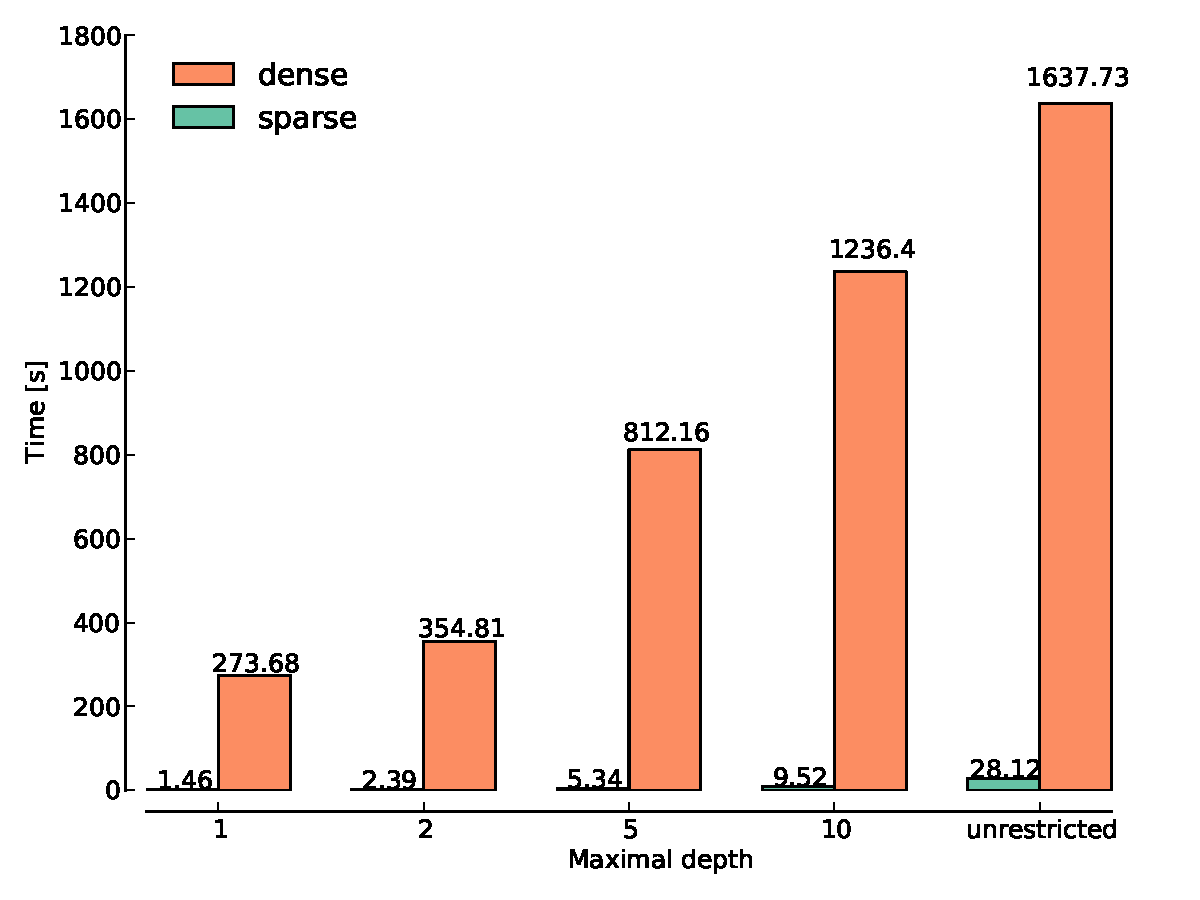
\includegraphics[scale=0.45]{images/20news.pdf}
\caption{Leveraging the input sparsity significantly speed up decisions
         tree induction both with shallow and deep trees on the \emph{20 Newsgroups}
         dataset. Note that the dataset is very sparse (density = 0.001).}
\label{fig:20news}
\end{figure}

\begin{figure}[h]
\centering
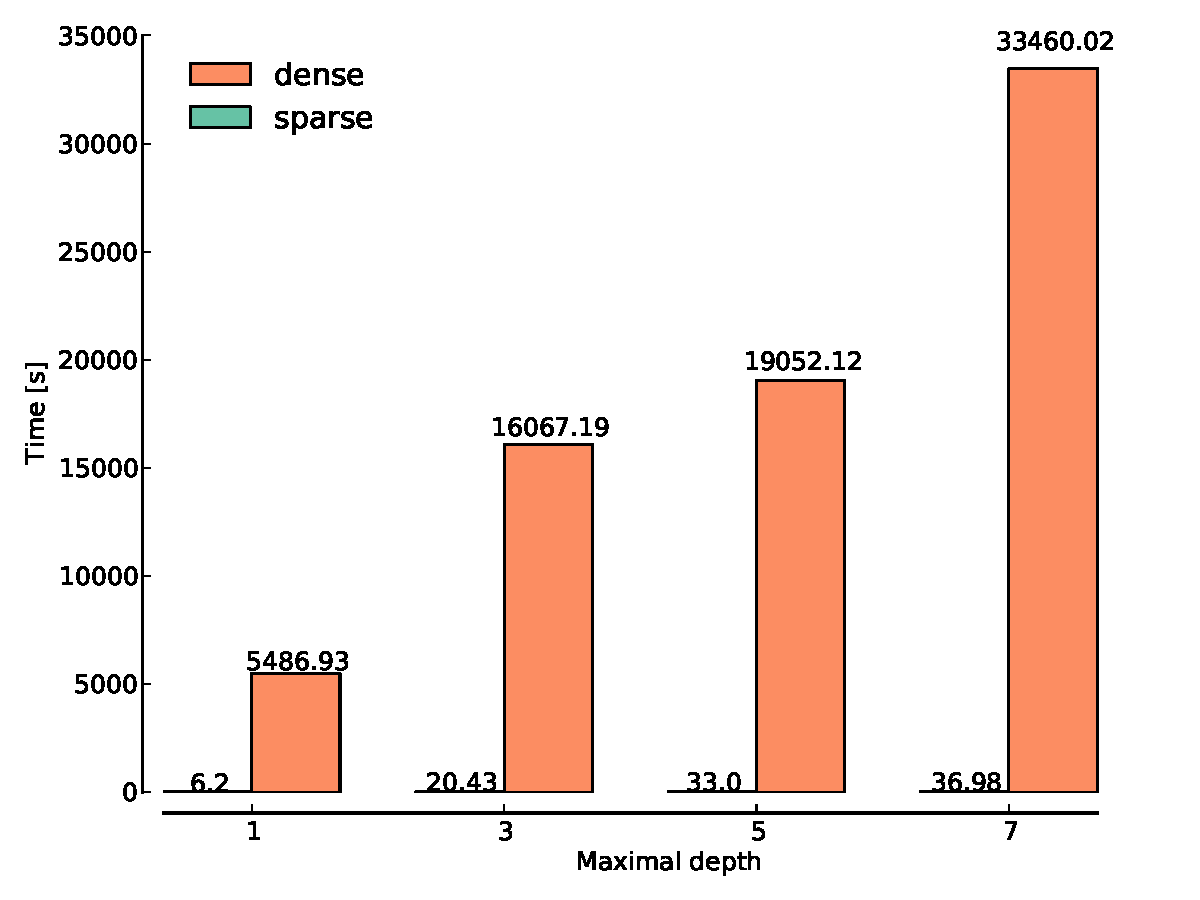
\includegraphics[scale=0.45]{images/cup.pdf}
\caption{Leveraging the input sparsity significantly speed up decisions
         tree induction both with shallow and deep trees on the \emph{cup}
         dataset. Note that the dataset is quite sparse (density = 0.014).}
\label{fig:cup}
\end{figure}


\begin{figure}[h]
\centering
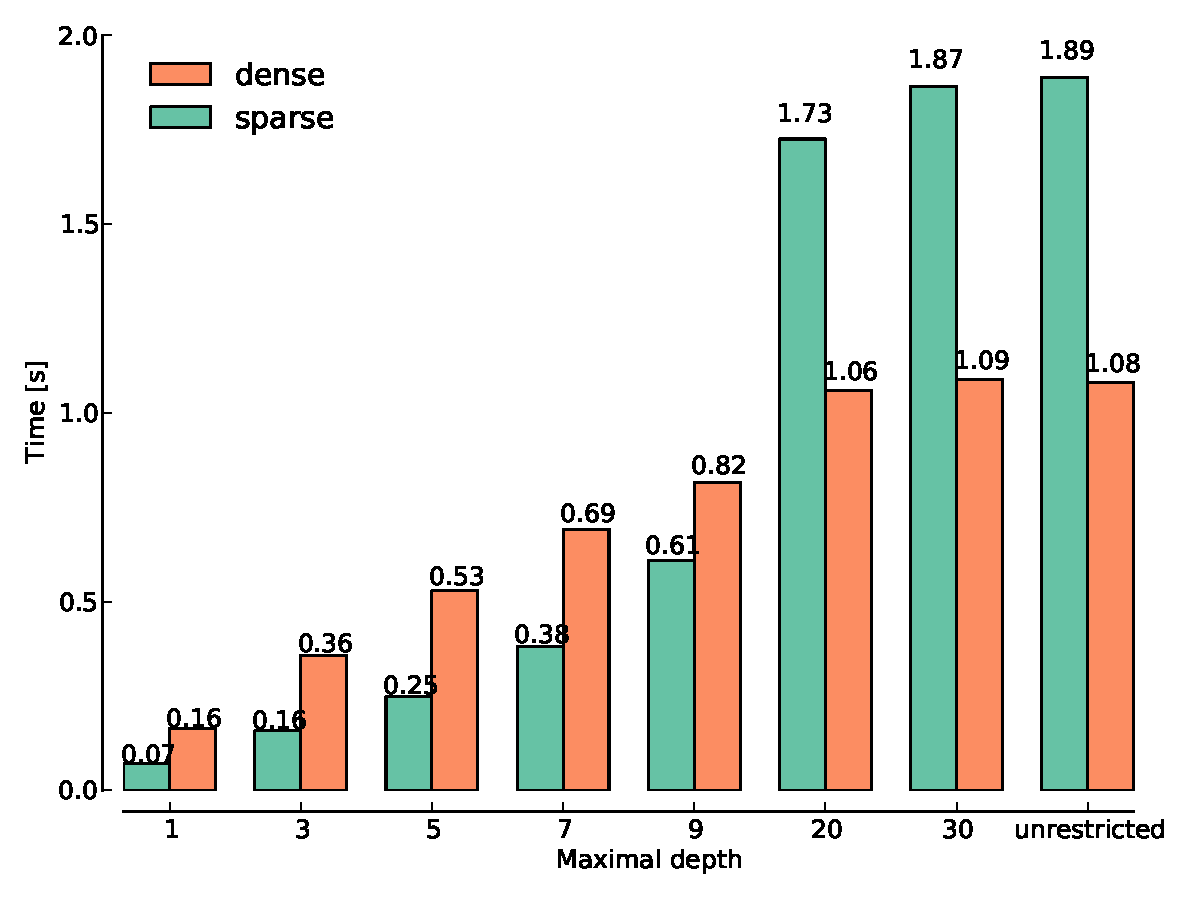
\includegraphics[scale=0.45]{images/adult.pdf}
\caption{Leveraging the input sparsity does not speed up training of deep trees on the \emph{adult}
         dataset. Note that the dataset is quite dense (density = 0.11).}
\label{fig:adult}
\end{figure}


\begin{figure}[h]
\centering
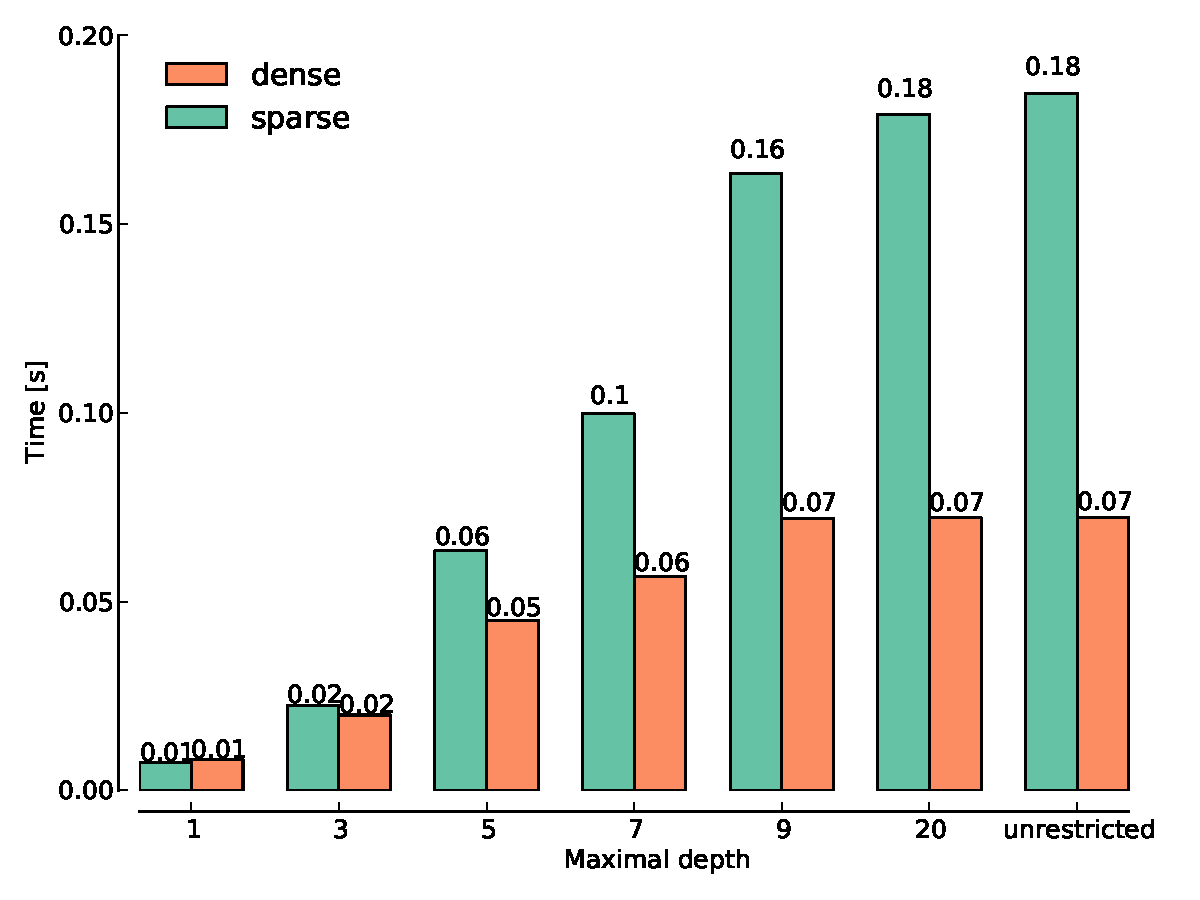
\includegraphics[scale=0.45]{images/tic.pdf}
\caption{Leveraging the input sparsity does not speed up training trees on the \emph{tic}
         dataset. Note that the dataset is very dense (density = 0.44).}
\label{fig:tic}
\end{figure}

In this section we will assess the computational performance of the decision tree algorithm on datasets composed dominantly of categorical or textual features, which makes them very sparse, and on datasets that are more dense. We will compare the learning time between the decision tree learnt
using a sparse csc matrix and a dense array.
The first two experiments are on very sparse datasets, namely on the \emph{20 Newsgroups} dataset \cite{joachims1996probabilistic} and on the \emph{KDD cup 1999} dataset\cite{bay2000archive}. The \emph{20 Newsgroups} dataset
consists of $n=11314$ document on $20$ topics. Each text document was
transformed into sparse tf-idf vectors of size $m=130107$ with a density of
$0.001$. \\
In tree-based ensemble methods, decision trees are either shallow trees as used
in boosting methods or deep trees as in random forest ensemble methods. Figure
\ref{fig:20news} shows that properly taking into account the sparsity of the
input space allows to speed up the learning from 58 times for a fully grown
tree up to 188 times for a decision stump. Furthermore, both algorithm leads
exactly to the same decision tree structure and have the same generalization
performance. The next dataset with low density is the \emph{KDD cup 1999} dataset which consists of $n=96367$ instances. The dataset contains both numerical and categorical data. The feature size of the dataset with categorical features transformed to binary features is $m=20025$ with an average density of
$0.014$. Unlike the previous dataset, the task at hand for this dataset is regression. We will compare the learning time between the decision tree regressor learnt
using a sparse csc matrix and a dense array. As Figure \ref{fig:cup} shows, taking into account the sparsity of the
input space allows to speed up the learning by a factor between 800 and 900. Furthermore, both algorithm lead
exactly to the same decision tree regressor structure and have the same generalization
performance.\\

Our dense datasets are the \emph{Adult} dataset\cite{Bache+Lichman:2013} with a density of $0.12$, $n=32561$ instances and  $m=145$ features, and the \emph{TIC} dataset\cite{Bache+Lichman:2013} with a density of $0.44$ and $n=4000$ instances and $m=85$ features. As Figure \ref{fig:adult} shows, for shallower trees sparse trees are approximately learnt twice faster than their dense counterparts, but for fully grown trees it is the opposite. Finally as Figure \ref{fig:tic} shows decision trees are learnt faster by dense input data rather than by input data sparsely represented. 


\subsection{Synthetic Data}

\begin{figure}[!h]
\centering
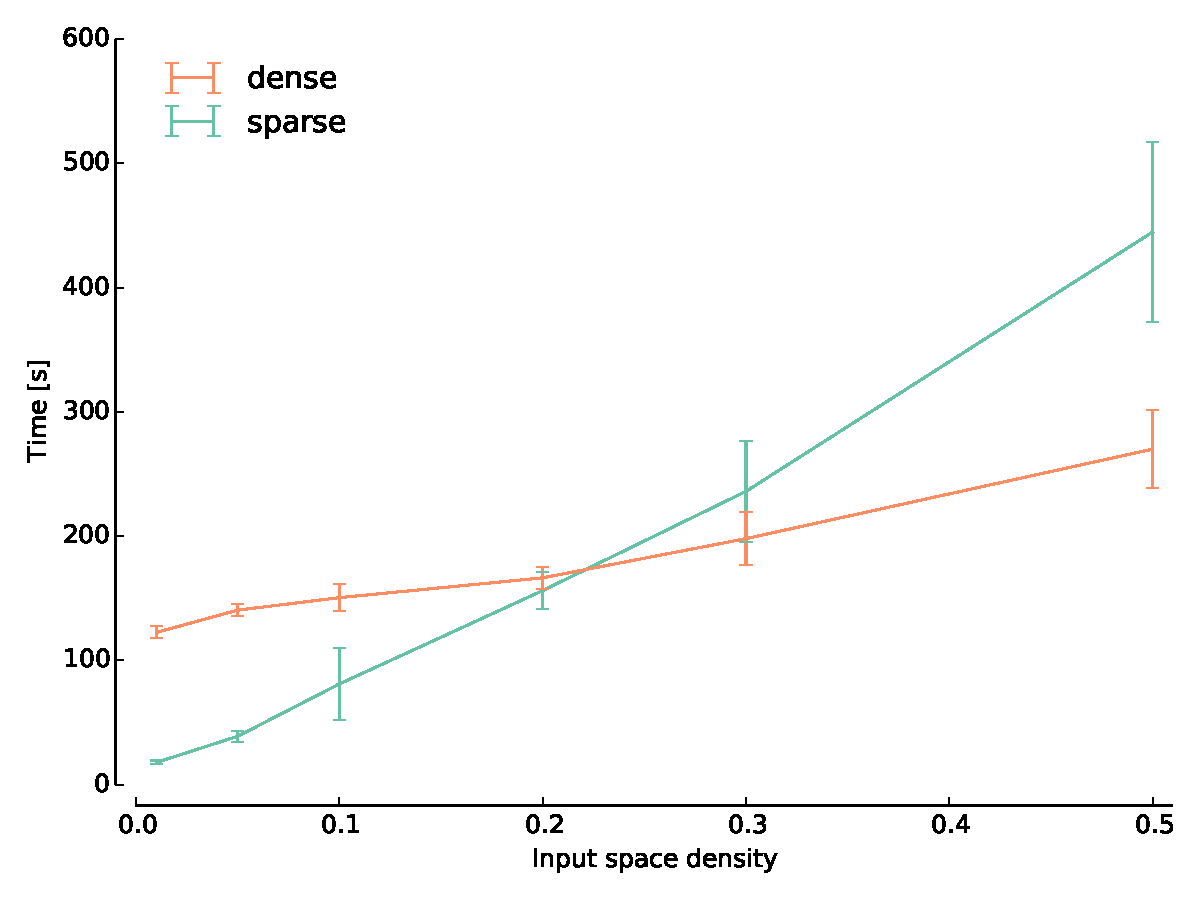
\includegraphics[scale=0.45]{images/density.pdf}
\caption{Significant speed up is achieved by the sparsity-aware decision tree
         algorithm whenever the density is below 0.2 (or sparsity over 0.8).}
\label{fig:density}
\end{figure}

As a another experiment, we generated random binary classification tasks with
$n=100000$ samples and $m=1000$ features. The input matrices are sparse random
matrices whose nonzero elements are drawn uniformly in $[0, 1)$. Their density
are ranging from $0.01$ to $0.5$. Each point is averaged over 20 experiments
and the maximal depth of the decision tree is restricted to 20. As illustrated
on Figure \ref{fig:density}, the sparsity aware decision tree induction
algorithm exploits the sparsity structure to be trained faster than its dense
counterpart. However whenever the input space density is over $0.2$, the
extraction of the nonzero values in the sparse csc matrix becomes expensive.
This suggests that the sparse decision tree induction algorithm is particularly
suited for sparsely representable data such as text documents.



%\begin{figure}[h]
%\centering
%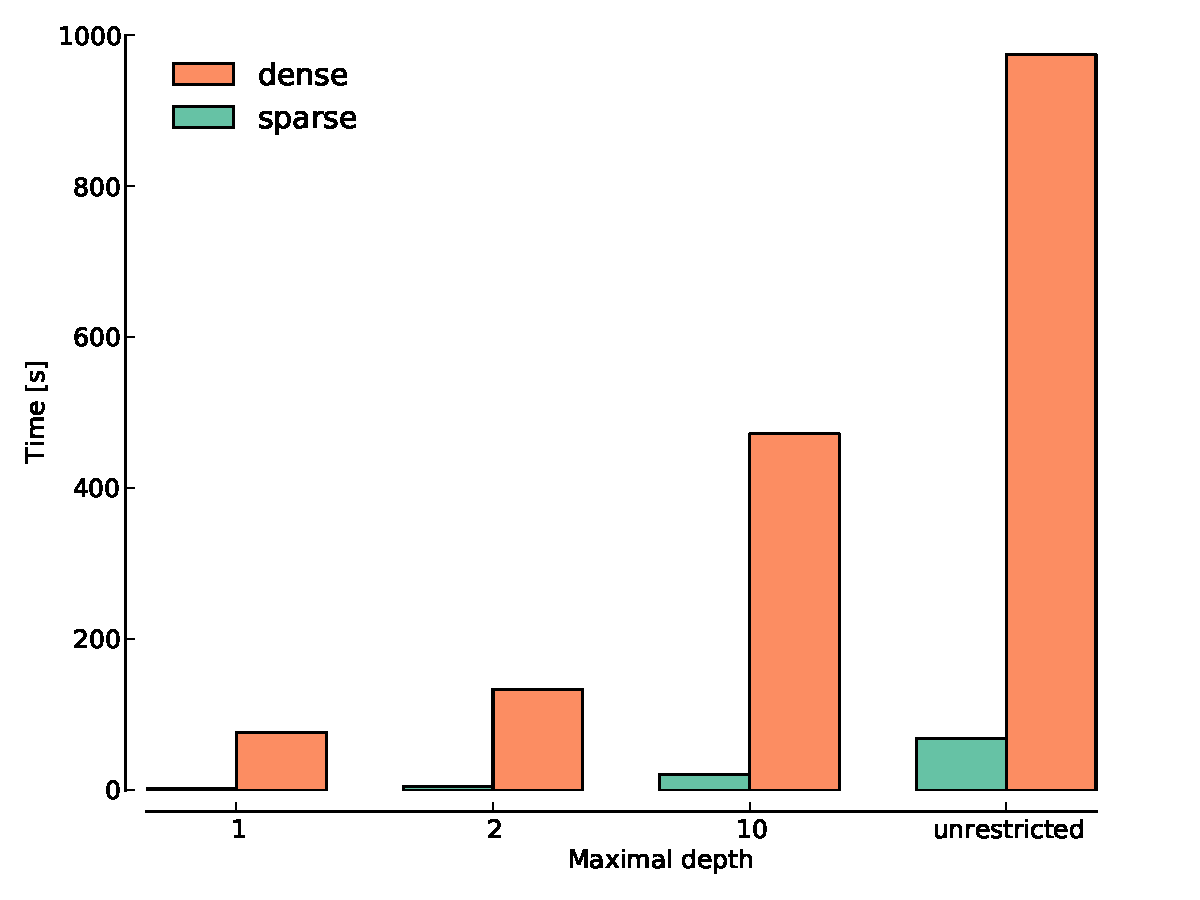
\includegraphics[scale=0.45]{images/depth.pdf}
%\caption{Leveraging the input sparsity significantly speed up decisions
%         tree induction both with shallow and deep trees on the \emph{20 Newsgroups}
%         dataset.}
%\label{fig:depth}
%\end{figure}




\section{Related Work}
\label{sec:related}

The main contribution of this paper is on scaling up tree-based models in presence of large and sparsely representable data. Many researchers in the field of machine learning and statistics have contributed to the development of decision tree-based algorithms and their ensemble variables such as random forests and AdaBoost. Hastie et al\cite{hastie:book2008}, Friedman et al \cite{breiman1984classification}, Quinlan \cite{Quinlan:1993:CPM:152181} and Shapire et al \cite{Schapire99improvedboosting} are some of the main contributors of the field. Their work however did not address scalability. Apache Mahout Spark MLlib is one of the only projects that addresses this issue. They train random forests by building multiple decision trees in parallel \cite{das:blog2014}. The individual trees however do no scale \cite{Zaharia:2010:SCC:1863103.1863113}. There are Scalable implementations of other machine learning algorithms such as SVM and Logistic Regression, and LibLinear \cite{Chang:2011:LLS:1961189.1961199} is a good example. With our algorithm incorporated into \emph{scikit-learn} \cite{buitinck2013api}, the open source now supports scalability of tree-based algorithms on sparsely representable data. 

. 

\section{Conclusion}
\label{sec:conclusion}
We proposed a method for building tree-based models with sparse input
support.  Our method takes advantage of input sparsity by avoiding
sorting sample sets of a node along a feature unless they are nonzero
at that feature. This approach speeds up training substantially as
sorting is a costly but an essential and ubiquitous component of
tree-based models.


\section{Acknowledgment} 
Arnaud Joly is a research fellow of the FNRS, Belgium. This work is
partially supported by PASCAL2 and the IUAP DYSCO, initiated by the
Belgian State, Science Policy Office.\\


\bibliographystyle{abbrv}
\bibliography{references}  
%
%\bibliography{sigproc}  % sigproc.bib is the name of the Bibliography in this case
% You must have a proper ".bib" file
%  and remember to run:
% latex bibtex latex latex
% to resolve all references
%
% ACM needs 'a single self-contained file'!
%
%APPENDICES are optional
%\balancecolumns

\end{document}
